%!TEX root = nonabelions.tex

\chapter{Abstract anyon models}\label{anyon models}

In this chapter we shall present the framework of abstract anyon models, leading up to the succeeding chapter that characterizes braiding of anyons described by abstract anyon models.

Anyon models can be modeled by unitary braided tensor categories, see \cite{kitaev}, one of the founding papers, and \cite{naaijkens,prakash,tensor categories,tuba}. However, setting up this framework in full generality is redundant for our purposes and we take a more straight forward approach, which is also most common in the literature. The benefit of the categorical approach is that consistency of braiding and fusion is most naturally shown this way. We shall see the ties between the straight forward approach and the categorical model in when discussing the consistency conditions in \cref{sec:pentagon hexagon}.

This chapter is in part based on \cite{preskill,kitaev,bonderson}. We shall be using the notation that is standard in the literature, and when possible make use of and extend the fusion diagram notation, which greatly clarifies braiding of fusion states.

Starting with \cref{sec:anyonic braid representations in fusion space} we show how a given abstract anyon model gives rise to representations of the braid group.

\section{Preliminaries}

An abstract anyon model consists of a set of labels representing different types of anyons. These labels are known as anyonic charge, topological charge or superselection labels. Anyons can be combined, or fused, to give an anyon of some charge, possibly in different ways. This is modeled by a fusion algebra
\begin{equation}
  a \times b = \sum_c N_{ab}^c c
\end{equation}
representing the possible outcomes from fusion of anyons of type $a$ and $b$. The fusion multiplicities $N_{ab}^c$ are non-negative integers denoting the number of distinct ways $a$ and $b$ can fuse to $c$. In each anyon model there is the trivial label $1$, representing the vacuum, with the property $N_{a1}^b = N_{1a}^b = \delta_{ab}$, i.e.\ $1$ fuses trivially with every other charge. Furthermore, to each charge $a$ there is a corresponding conjugate charge $\bar{a}$ representing the antiparticle of $a$, with the property $N_{ab}^1 = \delta_{b\bar{a}}$, i.e.\ $a$ fuses to the vacuum only with its antiparticle.

The $N_{ab}^c$ distinguishable ways in which $a$ and $b$ can fuse to $c$ can be regarded as an orthonormal basis of a Hilbert space $V_{ab}^c$. This is the state space, or fusion space, of anyons of type $c$ resulting from fusion of $a$ and $b$. The states of $V_{ab}^c$ are called fusion states and we denote the basis for $V_{ab}^c$ by
\begin{equation}
  \{ \ket{ab;c,\mu}, \quad \mu = 1,2,\ldots,N_{ab}^c \}
\end{equation}
where $\ket{ab;c,\mu}$ represents the $\mu$:th way in which $a$ and $b$ can fuse to $c$. This is the notation used by \cite{preskill}.

The splitting space $V_c^{ab}$ is the dual space of the fusion space $V_{ab}^c$, it is the state space of particles with anyonic charge $a$ and $b$ that can be split from an anyon of charge $c$.

More generally, the fusion space of anyons of type $c$ resulting from fusion of anyons of type $a_1, \ldots, a_n$ is denoted by $V_{a_1 a_2 \cdots a_n}^c$. This space has a canonical decomposition
\begin{equation}
  V_{a_1 a_2 \cdots a_n}^c \cong \bigoplus_{b_1,b_2,\ldots,b_{n-2}} V_{a_1a_2}^{b_1} \otimes V_{b_1 a_3}^{b_2} \otimes V_{b_2 a_4}^{b_3} \ldots \otimes V_{b_{n-2} a_n}^c
\end{equation}
with an associated canonical orthonormal basis with elements being the fusion states
\begin{equation}
  \ket{a_1 a_2; b_1, \mu_1} \otimes \ket{b_1 a_3; b_2, \mu_2} \otimes \cdots \otimes \ket{b_{n-3} a_{n-1}; b_{n-2}, \mu_{n-2}} \otimes \ket{b_{n-2} a_n; c, \mu_{n-1}}
\end{equation}
for all possible $b_j$ and $\mu_j$. For convenience we write $b_{0} = a_1$ and $b_{-1} = 1$.

Many anyon models of interest have the property that $N_{ab}^c \le 1$ for all particle types $a, b$ and $c$. When this is the case, such as for the Fibonacci anyons that we shall consider in \cref{fibonacci anyons}, the multiplicity label $\mu$ can be ignored. This makes the model easier to handle, and we introduce the fusion diagram notation.


\section{Fusion diagrams}

In the previous section we defined
\begin{equation}
  \ket{ab;c,μ}
\end{equation}
to represent the $μ$:th way in with $a$ and $b$ fuse to $c$. It shall be very convenient to use a diagrammatic notation for fusion states when considering braiding of anyons, as we shall see in the following sections. Thus, we introduce the notation
\begin{equation}
  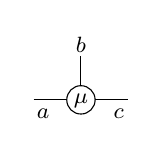
\begin{tikzpicture}[scale=0.4,font=\footnotesize,anchor=mid,baseline={([yshift=-.5ex]current bounding box.center)}]
    \node at (0, 1.7) {$b$};
    \draw (0, 1.4) to (0, 0.45);
    \draw (-1.5, 0) to (-0.45, 0);
    \draw (0.45, 0) to (1.5, 0);
    \draw (0, 0) circle (0.45);
    \node at (0.003, 0.08) {$\mu$};
    \node at (-1.2, -0.4) {$a$};
    \node at (1.2, -0.4) {$c$};
  \end{tikzpicture}
  \coloneqq \ket{ab;c;\mu}
\end{equation}
Note that the diagram should be read left/top to right/bottom, i.e.\ $a$ fuses with $b$ resulting in $c$.
For simplicity we suppress the multiplicity label $\mu$ in the notation and write
\begin{equation}
  \fs{b}{a,c} \coloneqq
  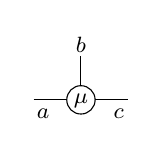
\begin{tikzpicture}[scale=0.4,font=\footnotesize,anchor=mid,baseline={([yshift=-.5ex]current bounding box.center)}]
    \node at (0, 1.7) {$b$};
    \draw (0, 1.4) to (0, 0.45);
    \draw (-1.5, 0) to (-0.45, 0);
    \draw (0.45, 0) to (1.5, 0);
    \draw (0, 0) circle (0.45);
    \node at (0.003, 0.08) {$\mu$};
    \node at (-1.2, -0.4) {$a$};
    \node at (1.2, -0.4) {$c$};
  \end{tikzpicture}
  \coloneqq \ket{ab;c;\mu}.
\end{equation}
This is convenient, since most models we shall consider are such that the fusion multiplicities are trivial, $N_{ab}^c \le 1$. That is, if fusion of $a$ and $b$ to $c$ is possible, this happens in exactly one way. Then, the multiplicity label $\mu$ in $\ket{ab;c,\mu}$ can be ignored, because the only possibility is $\mu = 1$, if $\mu=0$ the state is not valid. This is not a major simplification in the notation, it shall always be straight forward to add back the multiplicity labels if needed.

The diagram notation is primarily useful when considering fusion of several anyons and extends naturally;
\begin{equation}
  \fs{b,c}{a,e,d}
\end{equation}
denotes fusion of $a,b,c$ to $d$ such that $a$ fuses with $b$ resulting in the intermediate charge $e$, finally $e$ fuses with $c$ to give the resulting charge $d$.

The canonical basis for the fusion space $V_{a_1a_2\cdots a_n}^c$ with canonical decomposition
\begin{equation}
  V_{a_1 \cdots a_n}^c \cong \bigoplus_{b_1,b_2,\ldots,b_{n-2}} V_{a_1a_2}^{b_1} \otimes V_{b_1 a_3}^{b_2} \otimes V_{b_2 a_4}^{b_3} \ldots \otimes V_{b_{n-2} a_n}^c
\end{equation}
can thus be written in terms of fusion diagrams, assuming trivial fusion multiplicities, as
\begin{equation}
  \left\{
  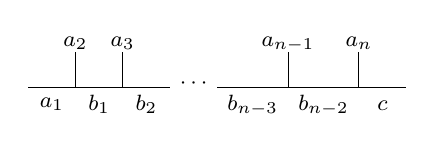
\begin{tikzpicture}[scale=0.3,font=\footnotesize,anchor=mid,baseline={([yshift=-.5ex]current bounding box.center)}]
    \node at (0, -0.6) {$a_1$};
    \node at (1, 2) {$a_2$};
    \node at (3, 2) {$a_3$};
    \node at (10, 2) {$a_{n-1}$};
    \node at (13, 2) {$a_n$};
%
    \draw (1, 0) to (1, 1.5);
    \draw (3, 0) to (3, 1.5);
%
    \draw (10, 0) to (10, 1.5);
    \draw (13, 0) to (13, 1.5);
%
    \draw (-1, 0) to (5, 0);
    \draw (7, 0) to (15, 0);
%
    \node at (2, -0.7) {$b_1$};
    \node at (4, -0.7) {$b_2$};
    \node at (6, 0.2) {$\cdots$};
%
    \node at (8.5, -0.7) {$b_{n-3}$};
    \node at (11.5, -0.7) {$b_{n-2}$};
    \node at (14, -0.7) {$c$};
  \end{tikzpicture}
  \;\;\;\bigg|\; \begin{array}{c}\text{for all possible intermediate} \\ \text{charges $b_1, b_2, \ldots, b_{n-2}$}\end{array}
  \right\}.
\end{equation}
It is thus clear that for given anyons $a_1, \ldots, a_n$ the fusion states are really determined by the intermediate charges $b_j$.

The real advantage of writing fusions states with fusion diagrams is that braiding is much easier to represent. This will be extremely useful now as we proceed in developing the abstract model for anyons, and characterize braiding.

Consider an arbitrary fusion state $\ket{\psi} = \sum_k c_k \ket{k}$ where $\ket{k}$ denotes the $k$:th basis fusion states. Let $A$ be a linear operator on the fusion space. The basis fusion states are transformed according to
\begin{equation}\label{eq:linear op on basis state}
  A\ket{k} = \sum_j A_{jk} \ket{j}
\end{equation}
The action of a linear operator $A$ acting on $\ket{\psi}$ is then given by
\begin{equation}
  A \ket{\psi} = \sum_k c_k A \ket{k} = \sum_{k} c_k \sum_j A_{jk} \ket{j} = \sum_j \sum_k c_k A_{jk} \ket{j}.
\end{equation}
Alternatively, written in Dirac notation, using the resolution of identity $I = \sum_j \ket{j}\bra{j}$, we have
\begin{equation}
  A \ket{\psi} = \sum_{j,k} \ket{j} \underbrace{\bra{j} A \ket{k}}_{A_{jk}} \underbrace{\braket{k}{\psi}}_{c_k}
\end{equation}

In what follows, we shall define some important linear operators on fusion spaces. We shall define the operators in terms of their action on the standard fusion states, as in \cref{eq:linear op on basis state}.












\section{The \texorpdfstring{$F$}{F} operator: Associativity of fusion}

The result of fusing multiple anyons is required to be independent of which anyons are fused first. This is motivated by the physics as the conservation of the anyonic charge. Mathematically, this translates to requiring that fusion is associative,
\begin{equation}
  (a \times b) \times c = a \times (b \times c).
\end{equation}
This gives rise to a natural isomorphism between the two decompositions of the fusion space
\begin{equation}
  V_{abc}^d \cong
  \bigoplus_f V_{ab}^f \otimes V_{fc}^d
  \cong
  \bigoplus_e V_{bc}^e \otimes V_{ea}^d
  .
\end{equation}
In terms of fusion diagrams that is
\begin{equation}
  \bigoplus_f \fs{b,c}{a,f,d}
  \cong
  \bigoplus_e \fsfused{a}{b}{c}{e}{d}.
\end{equation}
The first decomposition should be understood as first fusing $a$ with $b$ in all possible ways giving an intermediate charge $f$, followed by fusing $c$ with $f$ to give the final charge $d$.
The second decomposition should be understood as first fusing $b$ with $c$ in all possible ways giving an intermediate charge $e$, followed by fusing $a$ with $e$ to give the final charge $d$.

The first of these two decompositions is referred to as the standard decomposition and the second is the fusion decomposition. We denote this isomorphism by
\begin{equation}
  F : \bigoplus_f V_{ab}^f \otimes V_{fc}^d \to \bigoplus_e V_{bc}^e \otimes V_{ae}^d
\end{equation}
and it can be represented by the $F$ matrix.

\begin{definition}
  The $F$ matrix $F_{abc}^c$ is given by
  \begin{equation}\label{F-matrix}
    F : \fs{b,c}{a,e,d} \mapsto \fsfused{a}{b}{c}{d}{e} = \sum_f \left(F_{abc}^d\right)_{fe} \fs{b,c}{a,f,d}.
  \end{equation}
\end{definition}

That is, the $F$-matrix is the change of basis matrix from the standard basis to the fused basis in the fusion space $V_{abc}^d$.

\begin{remark}[Implicit range for the index of summation]\label{rem:sum index range}
  In \cref{F-matrix} the summation index $f$ implicitly ranges over all possible labels in the given anyon model, with the obvious restriction that the corresponding fusion state in the summand is valid. That is, the summation index $f$ must be such that
  \begin{equation}
    \begin{aligned}
      a \times b &= f \\
      f \times c &= d.
    \end{aligned}
  \end{equation}
  Similarly, the label $e$ is restricted so that
  \begin{equation}
    \begin{aligned}
      b \times c &= e \\
      a \times e &= d.
    \end{aligned}
  \end{equation}
  In what follows we shall let the summation index be implicit in all sums with fusion states as summands.
\end{remark}

The following lemma will be useful when computing the $F$-matrix.

\begin{lemma}\label{res:F1}
  Consider the fusion space $V_{abc}^d$, when one of the particle types is trivial, i.e.\ $a,b,c$ or $d$ equals $1$, then $\dim V_{abc}^d = 1$, furthermore if $a,b$ or $c$ equals $1$, then the corresponding $F$-matrix $F_{abc}^d$ is trivial. Explicitly that is
  \begin{equation}
    \begin{aligned}
      F_{1bc}^d &= \left( F_{1bc}^d \right)_{bd} = 1, \\
      F_{a1c}^d &= \left( F_{a1c}^d \right)_{ac} = 1, \\
      F_{ab1}^d &= \left( F_{ab1}^d \right)_{db} = 1.
    \end{aligned}
  \end{equation}
\end{lemma}

\begin{proof}
  With $a = 1$ we have, by definition of the $F$-matrix,
  \begin{equation}
     \fsfused{1}{b}{c}{d}{e} = \sum_f \left(F_{1bc}^d \right)_{fe} \fs{b,c}{1,f,d}.
  \end{equation}
  From the fusion diagram on the right hand side we read out $1 \times b = f$ from the first fusion, this is valid only for $f = b$.
  Similarly, on the left hand side the final fusion reads $1 \times e = d$, implying $e = d$. Since the indices $e$ and $f$ are forced, this implicitly shows that the corresponding fusion spaces is one-dimensional. The other results follow analogously,
  \begin{equation}
    \begin{aligned}
      \fsfused{a}{1}{c}{d}{e} &= \sum_f \left(F_{a1c}^d \right)_{fe} \fs{1,c}{a,f,d} \implies e = c, f = a, \\
      \fsfused{a}{b}{1}{d}{e} &= \sum_f \left(F_{ab1}^d \right)_{fe} \fs{b,1}{a,f,d} \implies e = b, f = d.
    \end{aligned}
  \end{equation}
  The result can also be realized by noting that three anyons of type $a, b$ and $c$, where one of them is the trivial type $1$, is uniquely determined by their total charge. Indeed, these three anyons are really just two, since the trivial particle $1$ fuses trivially, it can be added or removed in the representation without changing anything. Thus, the corresponding $F$ matrix must be trivial in this case. In particular, if $c = 1$, then
  \begin{equation}
    F_{a1c}ᵈ : \fs{b,1}{a,,d} ↦ \fsfused{a}{b}{1}{d}{}
  \end{equation}
  but
  \begin{equation}
    \fs{b,1}{a,,d} = \fs{b}{a,d} = \fsfused{a}{b}{1}{d}{}
  \end{equation}
  because the vacuum fuses trivially. Finally, the $F$-operator does a priori act non-trivially in these one-dimensional fusion spaces. However, one imposes the physical axiom that fusion and splitting with the vacuum is trivial. This can also be dealt with as a gauge choice in defining the standard basis states \cite{bonderson}.
\end{proof}















\section{The \texorpdfstring{$R$}{R} operator: Commutativity of fusion}

The result of fusing $a$ with $b$ must be the same as fusing $b$ with $a$. That is, fusion is commutative,
\begin{equation}
  a \times b = b \times a.
\end{equation}
This gives rise to a natural isomorphism.
\begin{definition}
  The $R$ operator $R_{ab}$ is an isomorphism
  \begin{equation}\label{R-matrix}
    R_{ab} : V_{ba}^c \to V_{ab}^c
  \end{equation}
  such that
  \begin{equation}
    R_{ab} :
    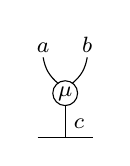
\begin{tikzpicture}[scale=0.35,font=\footnotesize,anchor=mid,baseline={([yshift=-.5ex]current bounding box.center)}]
      \node at (0.7, 2.7) {$a$};
      \node at (2.3, 2.7) {$b$};
      \draw (0.5, -0.6) to (2.5, -0.6);
      \draw (0.7, 2.3) to [bend left=-20] (1.25, 1.35);
      \draw (2.3, 2.3) to [bend left=20] (1.75, 1.35);
      \draw (1.5, 1) circle (0.45);
      \node at (1.503, 1.08) {$\mu$};
      \draw (1.5, 0.55) to (1.5, -0.6);
      \node at (2, -0.05) {$c$};
    \end{tikzpicture}
    \mapsto
    \begin{tikzpicture}[scale=0.3,font=\footnotesize,anchor=mid,baseline={([yshift=-.5ex]current bounding box.center)}]
      \node at (0.7, 4.9) {$a$};
      \node at (2.3, 4.9) {$b$};
      \braid[width=1.6cm, height=2cm] at (0.7, 4.5) s_1^{-1};
      \draw (0.5, -0.75) to (2.5, -0.75);
      \draw (0.7, 2) to [bend left=-30] (1.25, 1.2);
      \draw (2.3, 2) to [bend left=30] (1.75, 1.2);
      \draw (1.5, 0.85) circle (0.45);
      \node at (1.503, 0.9) {$\nu$};
      \draw (1.5, 0.4) to (1.5, -0.75);
      \node at (2, -0.15) {$c$};
    \end{tikzpicture}
    = \sum_{\nu} \left( R_{ab}^c \right)_{\nu\mu}
    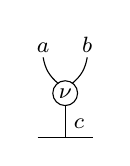
\begin{tikzpicture}[scale=0.35,font=\footnotesize,anchor=mid,baseline={([yshift=-.5ex]current bounding box.center)}]
      \node at (0.7, 2.7) {$a$};
      \node at (2.3, 2.7) {$b$};
      \draw (0.5, -0.6) to (2.5, -0.6);
      \draw (0.7, 2.3) to [bend left=-20] (1.25, 1.35);
      \draw (2.3, 2.3) to [bend left=20] (1.75, 1.35);
      \draw (1.5, 1) circle (0.45);
      \node at (1.503, 1.02) {$\nu$};
      \draw (1.5, 0.55) to (1.5, -0.6);
      \node at (2, -0.05) {$c$};
    \end{tikzpicture}.
  \end{equation}
  Disregarding the fusion multiplicities we see that the $R$ operator is diagonal,
  \begin{equation}
    R_{ab} : \fsfused{}{a}{b}{}{c} \mapsto \fsfusedbraided{}{a}{b}{}{c} = R_{ab}^c \fsfused{}{a}{b}{}{c}.
  \end{equation}
  That is, there is no mixing of the $c$ label. Note that mixing of $a$ and $b$ cannot occur since these are the charges to be braided and fused.
\end{definition}













\section{The \texorpdfstring{$B$}{B} operator: Braiding of standard fusion states}

We shall now consider braiding on the standard fusion states. This can be realized by applying the $F$-matrix to put the state in a basis where the $R$ matrix can be applied immediately, followed by reverting back to the standard basis via $F^{-1}$. That is, using the $F$ and $R$-matrix we obtain the relation
\begin{equation}
  \begin{aligned}
    \fs[1]{b,c}{a,e,d}
    &= \sum_f \left(\left(F^{-1}\right)_{acb}^d\right)_{fe} \fsfusedbraided{a}{b}{c}{d}{f} \\
    &= \sum_f \left(\left(F^{-1}\right)_{acb}^d\right)_{fe} R_{bc}^f \fsfused{a}{b}{c}{d}{f} \\
    &= \sum_g \sum_f \left(\left(F^{-1}\right)_{acb}^d\right)_{fe} R_{bc}^f \left(F_{abc}^d\right)_{gf} \fs{b,c}{a,g,d}.
  \end{aligned}
\end{equation}
Recall the implicit summation index convention described in \cref{rem:sum index range}.
From this we define the $B$-matrix.
\begin{definition}\label{def:B}
  The $B$ matrix $B_{abc}^d$ is given by
  \begin{equation}
    \left(B_{abc}^d\right)_{eg} = \sum_f \left(\left(F^{-1}\right)_{acb}^d\right)_{ef} R_{bc}^f \left(F_{abc}^d\right)_{fg}.
  \end{equation}
  Symbolically we write this as
  \begin{equation}
    B = F^{-1} R F.
  \end{equation}
\end{definition}
To sum up, the $B$-matrix braids the standard fusion states according to
\begin{equation}
  \fs[1]{b,c}{a,e,d} = \sum_g \left(B_{abc}^d\right)_{ge} \fs{b,c}{a,g,d}.
\end{equation}

As a consequence of the definition of the $B$-matrix and \cref{res:F1} we have the following lemma, which will be useful when computing the $B$-matrix.

\begin{lemma}\label{res:B1}
  Consider the fusion space $V_{abc}^d$, when one of the particle types is trivial, i.e.\ $a,b,c$ or $d$ equals $1$, then $\dim V_{abc}^d = 1$ and the corresponding $B$-matrix $B_{abc}^d$ is one-dimensional,
  \begin{equation}
    \begin{aligned}
      B_{1bc}^d &= \left( B_{1bc}^d \right)_{bc} = R_{bc}^d, \\
      B_{a1c}^d &= \left( B_{a1c}^d \right)_{ad} = R_{1c}^c = 1, \\
      B_{ab1}^d &= \left( B_{ab1}^d \right)_{da} = R_{b1}^b = 1.
    \end{aligned}
  \end{equation}
\end{lemma}















































\section{The pentagon and hexagon equations}\label{sec:pentagon hexagon}

When considering an anyon model, it is ultimately the $B$ operator (braid operator) that describes how braiding affects the anyons. The $B$ operator gives the phase change introduced when braiding anyons. In the next chapter we shall explicitly see how the $B$ operator is used to characterize the braid group representation for anyon models. It is the braid group representation that is the relevant property both for the study the dynamics of anyons, but also for developing methods for quantum computation with anyons, known as topological quantum computation.

We have seen that the $B$-matrix is computed from the $F$ and $R$-matrices. These matrices are in turn determined by what is known as the pentagon equation
% \begin{equation}\label{eq:pentagon}
%   \left(F_{12c}^5\right)^d_a \left(F_{a34}^5\right)^c_b = \left(F_{234}^d\right)^c_e \left( F_{1e4}^5 \right)^d_b \left( F_{123}^b \right)^e_a
% \end{equation}
\begin{equation}\label{eq:pentagon}
  \left(F_{12c}^5\right)_{da} \left(F_{a34}^5\right)_{cb} = ∑ₑ\left(F_{234}^d\right)_{ce} \left( F_{1e4}^5 \right)_{db} \left( F_{123}^b \right)_{ea}
\end{equation}
and hexagon equation
\begin{equation}\label{eq:hexagon}
  R_{13}^c \left(F_{213}^4\right)_{ca} R_{12}^a = \sum_{b} \left(F_{231}^4\right)_{cb} R_{1b}^4 \left(F_{123}^4\right)_{ba}.
  % R_{ac}^g \left(F_{bac}^d\right)^g_e R_{ab}^e = \sum_{f} \left(F_{bca}^d\right)^g_f R_{af}^d \left(F_{abc}^d\right)^f_e.
\end{equation}
In these equations, all indices are taken as arbitrary particle labels. \cite{preskill}

These equations should be understood as coherence conditions for fusion and braiding. The diagrammatic version of these equations, found as commutative diagrams in \cref{fig:pentagon_diagram,fig:hexagon_space} and \cref{fig:pentagon_space,fig:hexagon_space} make the point clear, and shows that these equations are commutativity constraints for fusion and braiding. Indeed, the pentagon equation is the formal constraint for associativity of fusion,
\begin{equation}
  (a \times b) \times c = a \times (b \times c).
\end{equation}
As previously hinted, anyon models can be described by braided tensor categories. In this setting, the pentagon and hexagon equations are precisely Mac Lane's coherence theorem \cite{mac lane}, showing that no further conditions are required for consistent fusion and braiding. Further details can be found in \cite{kitaev,preskill}.

Solving the pentagon and hexagon equations is in general highly non-trivial. The equations are multivariate polynomial equations and require elaborate techniques to be solved. First one must fix the gauge freedom that comes from the choice of basis for the fusion space, next an appropriate Gröbner basis can be used to solve the system. See \cite{bonderson} for more details on this approach.

\begin{figure}[!htb]
  \centering
  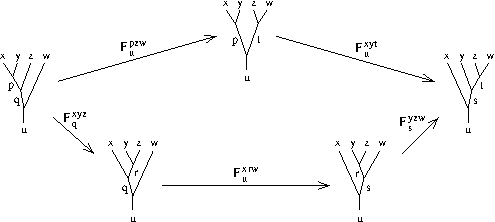
\includegraphics[width=1\linewidth]{img/pentagon_diagram.pdf}
  \caption{The pentagon equation in terms of fusion diagrams. Figure take from \cite{kitaev}. Note that the $F$-matrix have super- and sub-scripts reversed.}
  \label{fig:pentagon_diagram}
\end{figure}

\begin{figure}[!htb]
  \centering
  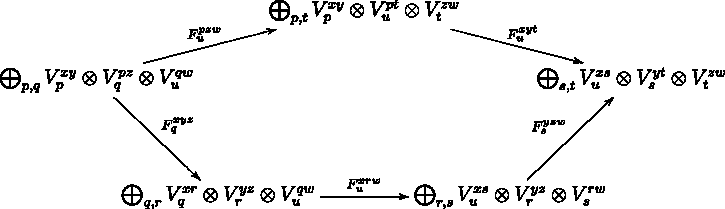
\includegraphics[width=1\linewidth]{img/pentagon_space.pdf}
  \caption{The pentagon equation in terms of fusion spaces. Figure take from \cite{kitaev}. Note that the fusion spaces and the $F$-matrix have super- and sub-scripts reversed.}
  \label{fig:pentagon_space}
\end{figure}

\begin{figure}[!htb]
  \centering
  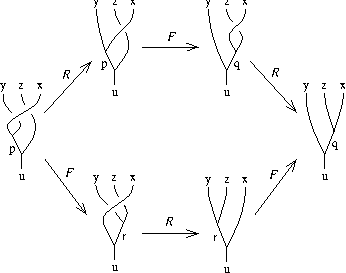
\includegraphics[width=0.8\linewidth]{img/hexagon_diagram.pdf}
  \caption{The hexagon equation in terms of fusion diagrams. Figure take from \cite{kitaev}.}
  \label{fig:hexagon_diagram}
\end{figure}

\begin{figure}[!htb]
  \centering
  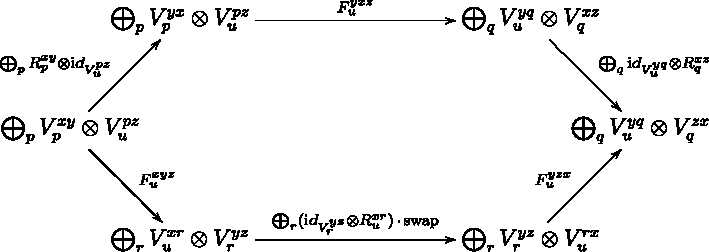
\includegraphics[width=1\linewidth]{img/hexagon_space.pdf}
  \caption{The hexagon equation in terms of fusion spaces. Figure take from \cite{kitaev}. Note that the fusion spaces, $F$-matrix and $R$-matrix have super- and sub-scripts reversed.}
  \label{fig:hexagon_space}
\end{figure}


\clearpage


